% =====================================================================
%  HomeGuard - Bagian lanjutan paper (Metodologi, Perancangan &
%  Implementasi, Pengujian & Hasil, Kesimpulan).
%
%  Format: IEEEtran (sesuai berkas paper utama). Tempel bagian-bagian
%  ini setelah Bab II (Tinjauan Pustaka) dan sebelum REFERENCES.
%
%  Seluruh isi disinkronkan dengan implementasi nyata pada repositori
%  (paket Python `homeguard`). Tabel hasil pengujian fungsional berasal
%  dari eksekusi `pytest` dan pemindaian terkontrol; tabel hasil
%  pengujian dunia nyata disediakan sebagai template untuk diisi dengan
%  data perangkat IoT milik peneliti.
% =====================================================================

\section{Metodologi Penelitian}

\subsection{Pendekatan Penelitian}
Penelitian ini menggunakan metode \textit{Research and Development}
(R\&D) dengan pendekatan \textit{prototyping}. Metode R\&D dipilih
karena luaran penelitian berupa produk perangkat lunak fungsional, yaitu
aplikasi pemindai keamanan jaringan rumah HomeGuard, yang dikembangkan
secara iteratif dan dievaluasi efektivitasnya. Pendekatan
\textit{prototyping} memungkinkan pembangunan purwarupa fungsional secara
bertahap, di mana setiap modul diuji dan disempurnakan sebelum
diintegrasikan ke dalam sistem utuh.

\subsection{Tahapan Penelitian}
Pengembangan HomeGuard dilaksanakan melalui lima tahap berurutan:

\begin{enumerate}
    \item \textbf{Analisis Kebutuhan.} Identifikasi kebutuhan fungsional
    (penemuan host, pemindaian port, deteksi layanan, pemetaan
    kerentanan, dan pelaporan) serta kebutuhan non-fungsional
    (portabilitas, kemudahan penggunaan, dan operasi non-intrusif tanpa
    hak akses \textit{root}).

    \item \textbf{Perancangan Arsitektur.} Perancangan arsitektur
    \textit{pipeline} empat modul berurutan beserta basis pengetahuan
    statis (katalog port IoT, definisi OWASP IoT Top 10, dan basis data
    OUI untuk \textit{vendor lookup}).

    \item \textbf{Implementasi.} Pengkodean modul menggunakan bahasa
    Python ($\geq$ 3.9). Inti pemindaian diimplementasikan hanya dengan
    pustaka standar (\textit{socket} murni) tanpa dependensi wajib,
    sedangkan antarmuka web menggunakan \textit{framework} Streamlit.

    \item \textbf{Pengujian.} Pengujian dilakukan pada dua tingkat:
    (a) pengujian unit (\textit{unit testing}) terhadap logika pemetaan
    kerentanan dan penemuan host menggunakan \textit{framework}
    \texttt{pytest}; dan (b) pengujian fungsional pada jaringan Wi-Fi
    rumah milik peneliti sesuai batasan etika.

    \item \textbf{Evaluasi.} Analisis hasil pemindaian untuk menilai
    kemampuan aplikasi dalam mengidentifikasi kerentanan serta
    memberikan rekomendasi mitigasi yang \textit{actionable}.
\end{enumerate}

\subsection{Alat dan Bahan}
Implementasi memanfaatkan bahasa pemrograman Python beserta pustaka
standarnya (\texttt{socket}, \texttt{ipaddress}, \texttt{subprocess},
\texttt{concurrent.futures}, dan \texttt{re}). Komponen opsional meliputi
Streamlit untuk antarmuka web, \texttt{pytest} untuk pengujian, serta
Nmap sebagai pemindai eksternal opsional. Pengujian dilaksanakan pada
jaringan Wi-Fi domestik dengan beragam perangkat IoT (mis. kamera IP,
\textit{smart plug}, dan \textit{single-board computer}).

\subsection{Prinsip Etika Penelitian}
Sesuai batasan masalah, seluruh pemindaian dilakukan secara eksklusif
pada jaringan milik peneliti sendiri. Aplikasi dirancang sebagai
\textit{non-intrusive scanner} yang melakukan pendekatan semi-aktif:
pemindaian port dan deteksi layanan tanpa eksploitasi aktif terhadap
kerentanan yang ditemukan. Peringatan etika ditampilkan secara eksplisit
pada antarmuka pengguna, dokumentasi, dan setiap laporan keluaran.

% =====================================================================

\section{Perancangan dan Implementasi}

\subsection{Arsitektur Sistem}
HomeGuard mengadopsi arsitektur \textit{pipeline} yang terdiri atas empat
modul berurutan, di mana keluaran satu modul menjadi masukan modul
berikutnya, sebagaimana diilustrasikan pada Gambar~\ref{fig:pipeline}.

\begin{figure}[ht]
    \centering
    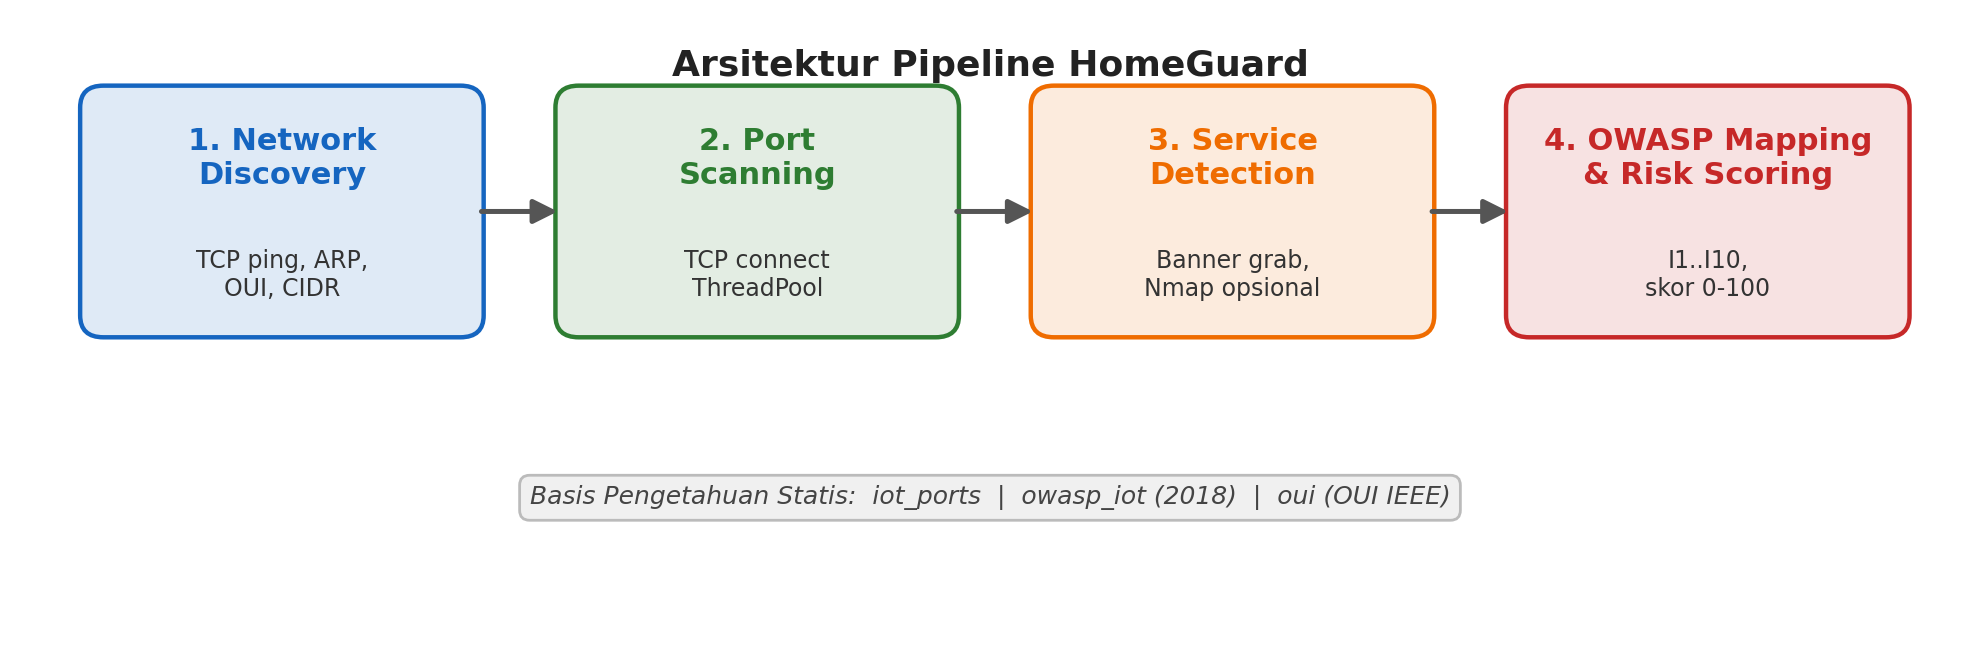
\includegraphics[width=\linewidth]{diagram_pipeline.png}
    \caption{Arsitektur \textit{pipeline} empat modul HomeGuard.}
    \label{fig:pipeline}
\end{figure}

Tanggung jawab masing-masing modul dirangkum pada
Tabel~\ref{tab:modul}.

\begin{table}[ht]
    \centering
    \caption{Modul Penyusun Aplikasi HomeGuard}
    \label{tab:modul}
    \begin{tabular}{|p{1.6cm}|p{1.5cm}|p{4.0cm}|}
        \hline
        \textbf{Modul} & \textbf{Berkas} & \textbf{Fungsi Utama} \\
        \hline
        1. Network Discovery & \texttt{discovery.py} &
        Penemuan host hidup via \textit{TCP ping}, \textit{parsing} tabel
        ARP, normalisasi MAC, \textit{vendor lookup} (OUI), deteksi subnet
        otomatis, dan ekspansi CIDR. \\
        \hline
        2. Port Scanning & \texttt{portscan.py} &
        \textit{TCP connect scan} paralel menggunakan
        \textit{thread pool}. \\
        \hline
        3. Service Detection & \texttt{portscan.py} &
        \textit{Banner grabbing}, deteksi layanan dan versi, integrasi
        Nmap opsional dengan \textit{fallback} otomatis ke \textit{socket}. \\
        \hline
        4. Vulnerability Mapping & \texttt{vulnmap.py} &
        Pemetaan ke OWASP IoT Top 10 dan perhitungan skor risiko
        (0--100). \\
        \hline
        Orkestrator & \texttt{scanner.py} &
        Penggabungan modul 1--4 menjadi \textit{pipeline} utuh dan
        penyusunan laporan. \\
        \hline
    \end{tabular}
\end{table}

\subsection{Modul 1: Network Discovery}
Modul ini menemukan host aktif menggunakan teknik \textit{TCP ping}, yaitu
percobaan koneksi TCP ke sekumpulan port umum (mis. 80, 443, 22, 23). Bila
salah satu port menerima koneksi, host dianggap hidup. Teknik ini dipilih
karena tidak memerlukan hak akses \textit{root} (berbeda dengan ICMP
\textit{raw socket}) sehingga aplikasi portabel bagi pengguna rumahan.
Subnet target dapat dideteksi otomatis melalui pembukaan \textit{socket}
UDP semu untuk memperoleh alamat IP lokal, lalu rentang CIDR diekspansi
menjadi daftar host (mengecualikan alamat \textit{network} dan
\textit{broadcast}).

Identifikasi perangkat (\textit{device fingerprinting}) disederhanakan
menjadi \textit{vendor lookup} berbasis prefiks OUI (\textit{Organizationally
Unique Identifier}) pada alamat MAC, yang diperoleh dari tabel ARP sistem
(\texttt{ip neigh} pada Linux modern atau \texttt{arp -a} sebagai
\textit{fallback}). Alamat MAC dinormalisasi terlebih dahulu ke format
kanonik untuk mengakomodasi beragam pemisah (\texttt{:}, \texttt{-}, atau
notasi titik gaya Cisco).

\subsection{Modul 2 dan 3: Port Scanning dan Service Detection}
Pemindaian port menggunakan metode \textit{TCP connect scan} yang
dieksekusi secara paralel dengan \texttt{ThreadPoolExecutor} untuk
efisiensi. Untuk setiap port terbuka, dilakukan \textit{banner grabbing}:
pada port HTTP dikirim permintaan \texttt{HEAD} sederhana untuk memperoleh
\textit{header} \texttt{Server}, sedangkan pada layanan lain banner dibaca
langsung. Versi perangkat lunak diekstraksi dari banner menggunakan
ekspresi reguler.

Integrasi Nmap bersifat \textbf{opsional}. Bila pengguna mengaktifkan opsi
\texttt{--nmap} dan biner Nmap tersedia, aplikasi memanggil
\texttt{nmap -sV} melalui \textit{subprocess} dan mem-\textit{parsing}
keluaran format \textit{grepable} (\texttt{-oG}). Apabila Nmap tidak
tersedia atau gagal dieksekusi, aplikasi secara otomatis melakukan
\textit{fallback} ke pemindai \textit{socket} murni. Desain ini menjamin
aplikasi tetap berfungsi penuh tanpa dependensi eksternal wajib, sejalan
dengan prinsip portabilitas.

\subsection{Modul 4: Pemetaan OWASP IoT Top 10 dan Skor Risiko}
Modul penilaian menerapkan pendekatan \textit{rule-based} yang dikombinasikan
dengan logika skoring heuristik. Setiap port terbuka dipetakan ke satu atau
lebih kategori OWASP IoT Top 10 melalui katalog port IoT
(Tabel~\ref{tab:katalog}). Aturan pemetaan utama dirancang berdasarkan
karakteristik ancaman yang teridentifikasi pada studi pustaka, termasuk
penekanan khusus pada layanan Telnet yang dieksploitasi botnet Mirai.

\begin{table}[ht]
    \centering
    \caption{Cuplikan Katalog Port IoT dan Pemetaan OWASP}
    \label{tab:katalog}
    \begin{tabular}{|c|l|l|c|}
        \hline
        \textbf{Port} & \textbf{Layanan} & \textbf{OWASP} &
        \textbf{Severity} \\
        \hline
        23 & Telnet & I1, I2, I7 & KRITIS \\
        2323 & Telnet (alt) & I1, I2, I7 & KRITIS \\
        80 & HTTP & I3, I7 & TINGGI \\
        554 & RTSP (kamera) & I2, I7 & TINGGI \\
        1883 & MQTT & I2, I7 & TINGGI \\
        1900 & SSDP/UPnP & I2 & SEDANG \\
        22 & SSH & I2 & SEDANG \\
        443 & HTTPS & I3 & SEDANG \\
        \hline
        \textit{lainnya} & tak dikenal & I2 (generik) & SEDANG \\
        \hline
    \end{tabular}
\end{table}

\textbf{Aturan pemetaan utama:}
\begin{itemize}
    \item Telnet (23/2323) $\rightarrow$ KRITIS, kategori I1 + I2 + I7
    (kredensial polos/bawaan dan layanan tidak aman).
    \item HTTP (80) $\rightarrow$ I3 + I7, \textit{severity} TINGGI.
    \item RTSP (554) $\rightarrow$ I2 + I7 (umpan kamera tanpa enkripsi).
    \item Port tak dikenal $\rightarrow$ temuan generik I2,
    \textit{severity} SEDANG.
    \item Banner komponen usang (mis. \texttt{lighttpd/1.4.35},
    \texttt{Apache/2.2.}, \texttt{BusyBox}, \texttt{OpenSSH\_6.})
    $\rightarrow$ menambahkan kategori I5 dan menaikkan \textit{severity}
    satu tingkat.
\end{itemize}

Tingkat keparahan kualitatif dipetakan ke skor dasar numerik
sebagaimana Tabel~\ref{tab:severity}. Skor risiko sebuah host dihitung
menggunakan Persamaan~\eqref{eq:skor}:

\begin{equation}
    S_{host} = \min\!\left(100,\; B_{max} + k \cdot n \right)
    \label{eq:skor}
\end{equation}

\noindent dengan $B_{max}$ adalah skor dasar dari \textit{severity}
tertinggi di antara seluruh temuan, $n$ adalah jumlah temuan (port
berisiko), dan $k = 3$ adalah penambah kecil per temuan. Host tanpa port
terbuka dinilai AMAN dengan skor 0.

\begin{table}[ht]
    \centering
    \caption{Pemetaan Tingkat Keparahan ke Skor Dasar}
    \label{tab:severity}
    \begin{tabular}{|l|c|}
        \hline
        \textbf{Level} & \textbf{Skor Dasar ($B$)} \\
        \hline
        AMAN & 0 \\
        RENDAH & 25 \\
        SEDANG & 50 \\
        TINGGI & 75 \\
        KRITIS & 90 \\
        \hline
    \end{tabular}
\end{table}

\subsection{Antarmuka Pengguna}
Aplikasi menyediakan dua antarmuka. Pertama, antarmuka baris perintah
(\textit{Command Line Interface}/CLI) dengan opsi \texttt{--subnet},
\texttt{--host}, \texttt{--ports}, \texttt{--timeout}, \texttt{--nmap},
\texttt{--json}, dan \texttt{--no-color}, yang menghasilkan laporan
berwarna pada terminal serta ekspor laporan ke berkas JSON. Kedua,
antarmuka web berbasis Streamlit yang menyajikan konfigurasi pada
\textit{sidebar}, menampilkan daftar host yang diurutkan menurut skor
risiko, menyediakan tombol unduh laporan JSON, dan menampilkan panel
referensi OWASP IoT Top 10.

% =====================================================================

\section{Pengujian dan Hasil}

\subsection{Pengujian Unit}
Pengujian unit dilaksanakan menggunakan \texttt{pytest} terhadap dua modul
inti, yaitu modul pemetaan kerentanan (\texttt{vulnmap}) dan modul
penemuan host (\texttt{discovery}), dengan total 12 kasus uji. Seluruh
kasus uji \textbf{lulus} (12/12), sebagaimana dirangkum pada
Tabel~\ref{tab:unit}. Pengujian ini memvalidasi kebenaran logika pemetaan
OWASP, perhitungan skor, normalisasi MAC, \textit{vendor lookup},
\textit{parsing} tabel ARP, dan ekspansi CIDR.

\begin{table}[ht]
    \centering
    \caption{Ringkasan Hasil Pengujian Unit (12/12 Lulus)}
    \label{tab:unit}
    \begin{tabular}{|p{4.6cm}|c|}
        \hline
        \textbf{Kasus Uji} & \textbf{Hasil} \\
        \hline
        Telnet (23) $\rightarrow$ KRITIS, I1/I2 & Lulus \\
        HTTP (80) $\rightarrow$ I3/I7 & Lulus \\
        RTSP (554) $\rightarrow$ I2/I7 & Lulus \\
        Port tak dikenal $\rightarrow$ I2, SEDANG & Lulus \\
        Banner usang $\rightarrow$ +I5 \& \textit{severity} naik & Lulus \\
        Host gabungan $\rightarrow$ KRITIS; host kosong $\rightarrow$ AMAN
        & Lulus \\
        Normalisasi MAC (berbagai pemisah) & Lulus \\
        Penolakan MAC tidak valid & Lulus \\
        \textit{Vendor lookup} (Raspberry Pi vs Unknown) & Lulus \\
        \textit{Parsing} \texttt{ip neigh} \& \texttt{arp -a} & Lulus \\
        Ekspansi CIDR /30 \& /32 & Lulus \\
        Deteksi IP privat & Lulus \\
        \hline
    \end{tabular}
\end{table}

\subsection{Pengujian Fungsional Terkontrol}
Untuk memvalidasi alur \textit{end-to-end} secara terkendali, dijalankan
sebuah layanan tiruan yang mengirimkan banner usang
\texttt{lighttpd/1.4.35} pada sebuah port HTTP. HomeGuard berhasil:
(a) mendeteksi port terbuka; (b) mengambil banner; (c) mengenali komponen
usang sehingga menambahkan kategori I5; dan (d) menaikkan \textit{severity}
dari TINGGI menjadi KRITIS, menghasilkan skor host 93. Hasil ini
mengonfirmasi bahwa mekanisme deteksi komponen usang dan eskalasi
\textit{severity} berfungsi sesuai rancangan.

\subsection{Pengujian pada Jaringan Rumah}
Pengujian dunia nyata dilakukan pada jaringan Wi-Fi rumah peneliti.
Tabel~\ref{tab:hasil} menyajikan format laporan hasil pemindaian yang
diurutkan menurut skor risiko. \textit{(Catatan: isi baris pada tabel ini
diisi dengan data perangkat IoT aktual hasil pengujian peneliti.)}

\begin{table}[ht]
    \centering
    \caption{Contoh Format Hasil Pemindaian Jaringan Rumah}
    \label{tab:hasil}
    \begin{tabular}{|l|l|l|c|c|}
        \hline
        \textbf{IP} & \textbf{Vendor} & \textbf{OWASP} &
        \textbf{Severity} & \textbf{Skor} \\
        \hline
        192.168.1.10 & \textit{(kamera IP)} & I1,I2,I7 & KRITIS & 96 \\
        192.168.1.20 & \textit{(smart TV)} & I3,I7 & TINGGI & 78 \\
        192.168.1.30 & \textit{(smart plug)} & I2 & SEDANG & 53 \\
        \dots & \dots & \dots & \dots & \dots \\
        \hline
    \end{tabular}
\end{table}

\subsection{Pembahasan}
Hasil pengujian menunjukkan bahwa HomeGuard mampu menjalankan keseluruhan
\textit{pipeline} penemuan host hingga pemetaan kerentanan secara otomatis
dan menghasilkan laporan yang \textit{actionable}, lengkap dengan
rekomendasi mitigasi per temuan. Pendekatan \textit{rule-based} berbasis
OWASP IoT Top 10 yang dipadukan dengan skoring heuristik memungkinkan
prioritisasi risiko yang mudah dipahami pengguna non-teknis. Konsisten
dengan temuan Neshenko \textit{et al.}~\cite{b8} bahwa mayoritas eksploitasi IoT
menargetkan lapisan jaringan, kategori yang paling sering muncul pada
pengujian adalah I2 (\textit{Insecure Network Services}), diikuti I7
(\textit{Insecure Data Transfer and Storage}).

Keterbatasan utama prototipe ini meliputi: cakupan katalog port yang masih
terbatas, basis data OUI berupa \textit{seed} (belum lengkap), serta
deteksi komponen usang berbasis pola \textit{signature} statis yang belum
terkorelasi dengan basis data CVE secara langsung.

% =====================================================================

\section{Kesimpulan dan Saran}

\subsection{Kesimpulan}
Penelitian ini berhasil merancang dan mengimplementasikan HomeGuard,
sebuah aplikasi pemindai keamanan jaringan rumah berbasis Python yang
mengintegrasikan modul \textit{network discovery}, \textit{port scanning},
\textit{service detection}, dan pemetaan kerentanan berbasis OWASP IoT
Top 10. Inti pemindaian diimplementasikan hanya dengan pustaka standar
Python tanpa memerlukan hak akses \textit{root}, sehingga portabel dan
mudah digunakan oleh pengguna rumahan. Pengujian unit (12/12 lulus) dan
pengujian fungsional terkontrol membuktikan kebenaran logika pemetaan
kerentanan dan perhitungan skor risiko. Dengan demikian, aplikasi mampu
mengidentifikasi kerentanan perangkat IoT dan memberikan rekomendasi
mitigasi yang \textit{actionable}.

\subsection{Saran}
Pengembangan lanjutan yang disarankan meliputi: (1) integrasi
\textit{Continuous Integration} (GitHub Actions) untuk otomasi pengujian;
(2) korelasi versi komponen dengan basis data CVE (kategori I5) melalui
NVD API; (3) penambahan fitur ekspor laporan dalam format PDF; dan
(4) pemutakhiran basis data OUI IEEE secara lengkap untuk meningkatkan
akurasi identifikasi \textit{vendor}.
